\documentclass[11pt]{report}

% Paquetes y configuraciones adicionales
\usepackage{amsmath, amsthm, amssymb} % Paquetes matemáticos
\usepackage[utf8]{inputenc} % Codificación .tex
\usepackage[T1]{fontenc} % Codificación .pdf
\usepackage{graphicx}
\usepackage[export]{adjustbox}
\usepackage{caption}
\usepackage{float}
\usepackage{titlesec}
\usepackage{geometry}
\usepackage[hidelinks]{hyperref}
\usepackage{titling}
\usepackage{titlesec}
\usepackage{parskip}
\usepackage{wasysym}
\usepackage{tikzsymbols}
\usepackage{fancyvrb}
\usepackage{xurl}
\usepackage{hyperref}
\usepackage{subcaption}
\usepackage{listings}
\usepackage{xcolor}
\usepackage[english]{babel}


\newcommand{\subtitle}[1]{
  \posttitle{
    \par\end{center}
    \begin{center}\large#1\end{center}
    \vskip0.5em}
}

% Configura los márgenes
\geometry{
  left=2cm,   % Ajusta este valor al margen izquierdo deseado
  right=2cm,  % Ajusta este valor al margen derecho deseado
  top=3cm,
  bottom=3cm,
}

% Configuración de los títulos de las secciones
\titlespacing{\section}{0pt}{\parskip}{\parskip}
\titlespacing{\subsection}{0pt}{\parskip}{\parskip}
\titlespacing{\subsubsection}{0pt}{\parskip}{\parskip}

% Redefinir el formato de los capítulos y añadir un punto después del número
\makeatletter
\renewcommand{\@makechapterhead}[1]{%
  \vspace*{0\p@} % Ajusta este valor para el espaciado deseado antes del título del capítulo
  {\parindent \z@ \raggedright \normalfont
    \ifnum \c@secnumdepth >\m@ne
        \huge\bfseries \thechapter.\ % Añade un punto después del número
    \fi
    \interlinepenalty\@M
    #1\par\nobreak
    \vspace{10pt} % Ajusta este valor para el espacio deseado después del título del capítulo
  }}
\makeatother

% Configura para que cada \chapter no comience en una pagina nueva
\makeatletter
\renewcommand\chapter{\@startsection{chapter}{0}{\z@}%
    {-3.5ex \@plus -1ex \@minus -.2ex}%
    {2.3ex \@plus.2ex}%
    {\normalfont\Large\bfseries}}
\makeatother

\definecolor{mygreen}{RGB}{0,128,0}  % Definir el color verde (0,128,0)
\definecolor{myblue}{RGB}{0,0,128}   % Definir el color azul (0,0,128)

\begin{document}

% Portada del informe
\title{Practice Report}
\subtitle{Robótica Computacional}
\author{Cheuk Kelly Ng Pante (alu0101364544@ull.edu.es)}
\date{\today}

\maketitle

\pagestyle{empty} % Desactiva la numeración de página para el índice

% Índice
\tableofcontents

% Nueva página
\newpage

\pagestyle{plain} % Vuelve a activar la numeración de página
\setcounter{page}{1} % Reinicia el contador de página a 1

% Secciones del informe
% Capitulo 1
\chapter{Forward kinematics}
Forward kinematics is a branch of robotics and mechanics that deals with the relationship between the movements
of the links of a robot and the variables that control them. In other words, forward kinematics is the problem
of finding the position and orientation of the end of the robot, given the set of parameters that define the 
positions and orientations of all the links.

To explain the forward kinematics, the Denavit-Hartenberg (DH) coordinate system will be used. The Denavit-Hartenberg 
coordinate system is a coordinate system used to model direct and inverse kinematics of articulated robots. The 
Denavit-Hartenberg coordinate system is based on four parameters associated with each joint. These parameters are:
\begin{itemize}
  \item $d_i$: Distance between the $z_{i-1}$ and $z_i$ axes along the $x_{i-1}$ axis.
  \item $\theta_i$: Angle between the $z_{i-1}$ and $z_i$ axes around the $x_{i-1}$ axis.
  \item $a_i$: Distance between the $x_{i-1}$ and $x_i$ axes along the $z_{i-1}$ axis.
  \item $\alpha_i$: Angle between the $x_{i-1}$ and $x_i$ axes around the $z_{i-1}$ axis.
\end{itemize}

The DH parameters can be calculated according to the following table:
\begin{table}[H]
  \centering
  \begin{tabular}{|c|c|c|c|}
    \hline
    \textbf{}           & \textbf{A}                 & \textbf{B}                 & \textbf{C}         \\ \hline
    \textbf{$d_i$}      & \texttt{$O_{i-1}$}         & \texttt{$Z_{i-1}\cap X_i$} & \texttt{$Z_{i-1}$} \\ \hline
    \textbf{$\theta_i$} & \texttt{$X_{i-1}$}         & \texttt{$X_{i}$}           & \texttt{$Z_{i-1}$} \\ \hline
    \textbf{$a_i$}      & \texttt{$Z_{i-1}\cap X_i$} & \texttt{$O_{i}$}           & \texttt{$X_{i}$}   \\ \hline
    \textbf{$\alpha_i$} & \texttt{$Z_{i-1}$}         & \texttt{$Z_{i}$}           & \texttt{$X_{i}$}   \\ \hline
  \end{tabular}
  \caption{Parameters of DH}
\end{table}

For the explanation of forward kinematics, manipulator 3 will be used:
\begin{figure}[H]
  \centering
  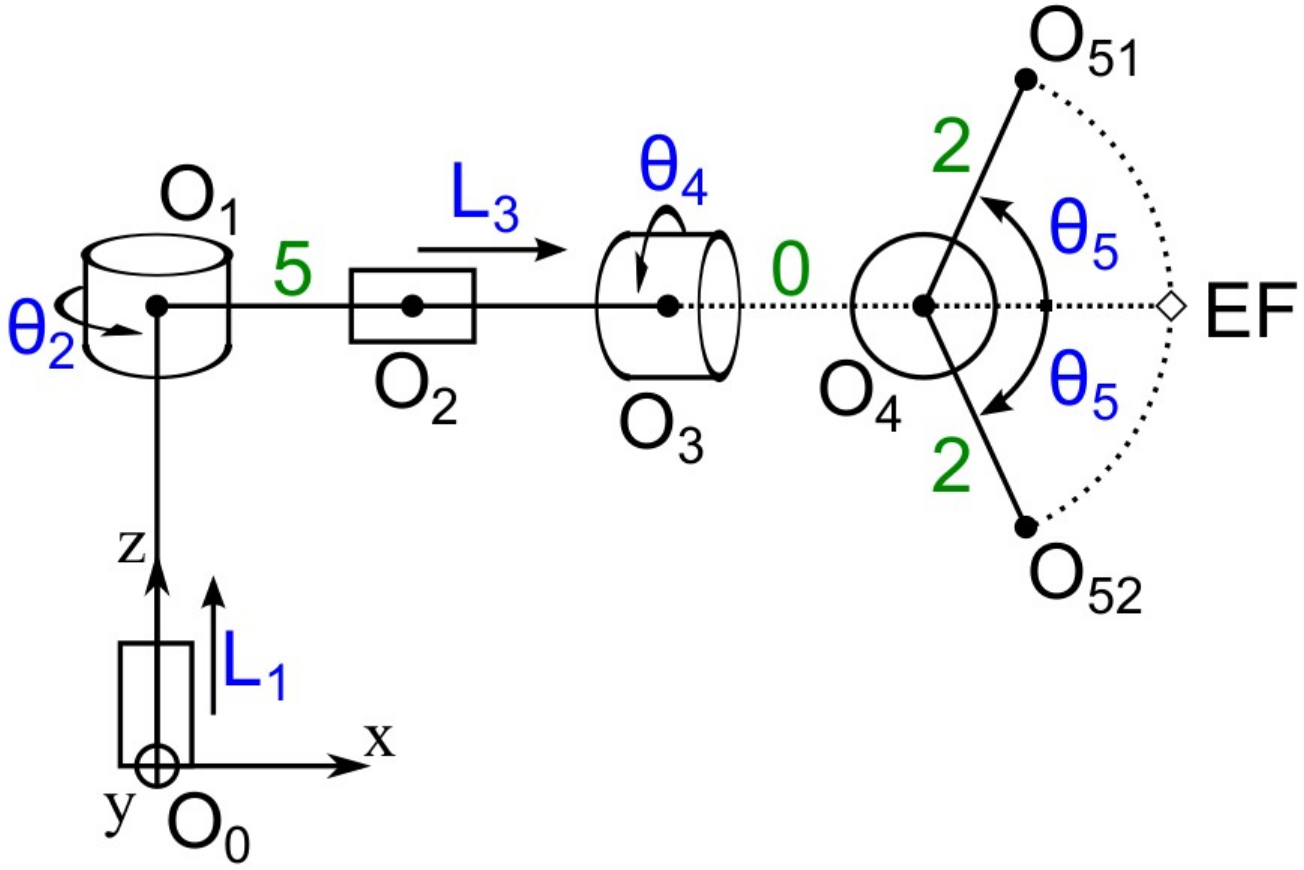
\includegraphics[scale=0.24]{img/manipulador.png}
  \caption{Example manipulator}
\end{figure}

To calculate the forward kinematics, we will first calculate the DH parameters:
\begin{figure}[H]
  \centering
  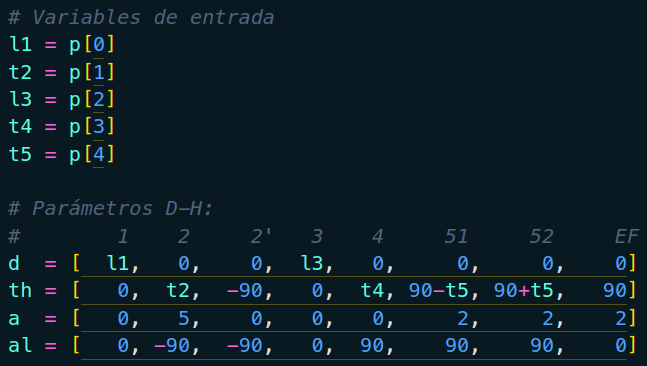
\includegraphics[scale=0.4]{img/parametros_dh.png}
  \caption{Manipulator 3 DH parameters}
\end{figure}

As can be seen in figure 1.2, before calculating the DH parameters, some input variables have been assigned, these 
correspond to the angles of the manipulator joints and these are the values that are introduced when the program is 
executed. For example, if we run it as follows:
\begin{verbatim}
$ python3 ./cinematica_directa 5 0 5 90 45
\end{verbatim}

the forward kinematics result would be:
\begin{figure}[H]
  \centering
  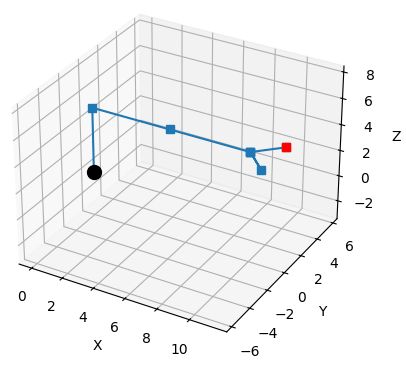
\includegraphics[scale=0.7]{img/cinematica_directa.png}
  \caption{Forward kinematics of manipulator 3}
\end{figure}

\newpage

Then, the transformation matrix of each joint was calculated for this manipulator:
\begin{figure}[H]
  \centering
  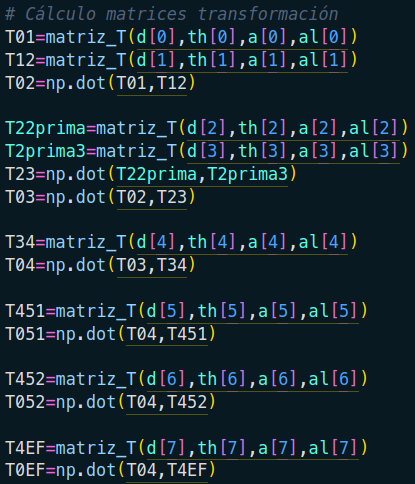
\includegraphics[scale=0.5]{img/matriz_transformacion.png}
  \caption{Matrix transformation of each joint of manipulator 3}
\end{figure}

Then, the transformation of each joint, specifying the data from the Denavit Hartenberg table specified in figure 1.2:
\begin{figure}[H]
  \centering
  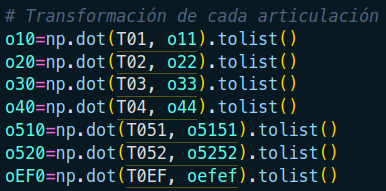
\includegraphics[scale=0.5]{img/transformacion_articulacion.png}
  \caption{Transformation of each manipulator joint 3}
\end{figure}

And finally, the result of the forward kinematics of manipulator 3:
\begin{figure}[H]
  \centering
  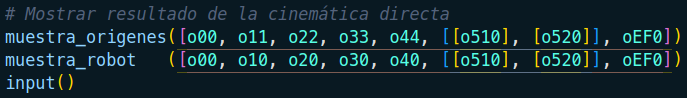
\includegraphics[scale=0.5]{img/resultado_cd.png}
  \caption{Result of the forward kinematics of manipulator 3}
\end{figure}

\newpage

\chapter{Inverse kinematics}
Inverse kinematics is a branch of robotics and mechanics that deals with the relationship between the movements of the
links of a robot and the variables that control them. In other words, inverse kinematics is the problem of finding the 
set of parameters that define the positions and orientations of all the links, given the position and orientation of 
the end of the robot.

Inverse kinematics can be a complex problem due to the presence of physical constraints and limitations of the robot, 
such as joint movement limits, collisions or singularities.

In the practice of inverse kinematics, the distance that a prismatic joint at point $O_i$ has to be extended in such a 
way that the end point of the robot $O_n$ is as close as possible to the target position R is to be calculated.

The approach can only be made in the extension direction $L_i$, which can be calculated as an angle of $w$ defining the
rotation with respect to the absolute x-axis. The angle $w$ can be calculated as:
\begin{equation*}
  \color{blue}\omega\color{black} = \sum_{j = 0}^{\color{blue}i\color{black}} \theta_j
\end{equation*}

Using the scalar product we can project the vector $O_n$ to $R$ in the direction of extension of the joint to obtain the distance $d$:
\begin{equation*}
  \color{green} \mathbf{d} \color{black} =
  \begin{bmatrix}
    \cos(\color{blue}\omega\color{black}) \\
    \sin(\color{blue}\omega\color{black})
  \end{bmatrix}
  \cdot (\color{red}R\color{black}- \color{red}\text{ON}\color{black})
\end{equation*}

Therefore, the value of $L_i$ after each iteration becomes:
\begin{equation*}
  \color{green} \mathbf{L_i} \color{black} +
  \begin{bmatrix}
    \cos(\color{blue}\omega\color{black}) \\
    \sin(\color{blue}\omega\color{black})
  \end{bmatrix}
  \cdot (\color{red}R\color{black}- \color{red}\text{ON}\color{black}),\ \ \ con \ 
  \color{blue}\omega\color{black} = \sum_{j = 0}^{\color{blue}i\color{black}} \theta_j
\end{equation*}

To calculate the inverse kinematics in the script in \emph{Python} we will do it with the Cyclic Coordinate Descent (CCD) algorithm. 
And before we start developing the CCD algorithm, we must first define the joint values for the direct kinematics.
For this purpose, lists have been defined with the joint values of each joint of the robot and these joint values 
have been defined so that the robot does not exceed the limits of the joints, upper and lower limits. And then, with 
another list, we will differentiate between a rotational joint and a prismatic joint.

\begin{figure}[H]
  \centering
  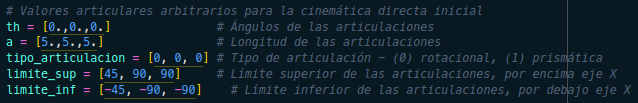
\includegraphics[scale=0.7]{img/listas_ci.png}
  \caption{Lists of limits joints articulations}
\end{figure}

\newpage

Then, already differentiating the joint values, in the main loop we compute $\omega$, which for the rotational joint 
we calculate the vectors $V_1$ and $V_2$, which represent the position differences between the points of interest. 
For vector $V_1$ is the difference between the robot end point and the target and for vector $V_2$ is the difference 
between the robot end point and the point of interest. Once the vectors are calculated, we calculate the angles between 
the vectors $V_1$ and $V_2$ and these angles are added to the variable $\theta$ of the rotational joint making the
difference between the angles of the vectors $V_1$ and $V_2$. And in the case of the prismatic joint it will be the sum 
of all the $\theta$ up to the current one (inclusive) and then the scalar projection of the vector that goes from the end 
point of the robot to the target on the extension direction of the prismatic joint is calculated.

Afterwards, it is necessary to ensure that the robot does not exceed the limits of the joints, so the current position must 
be checked to see if it is above or below the limits, and if so, the position will become that of the limit itself, whether 
it is above or below.
\begin{figure}[H]
  \centering
  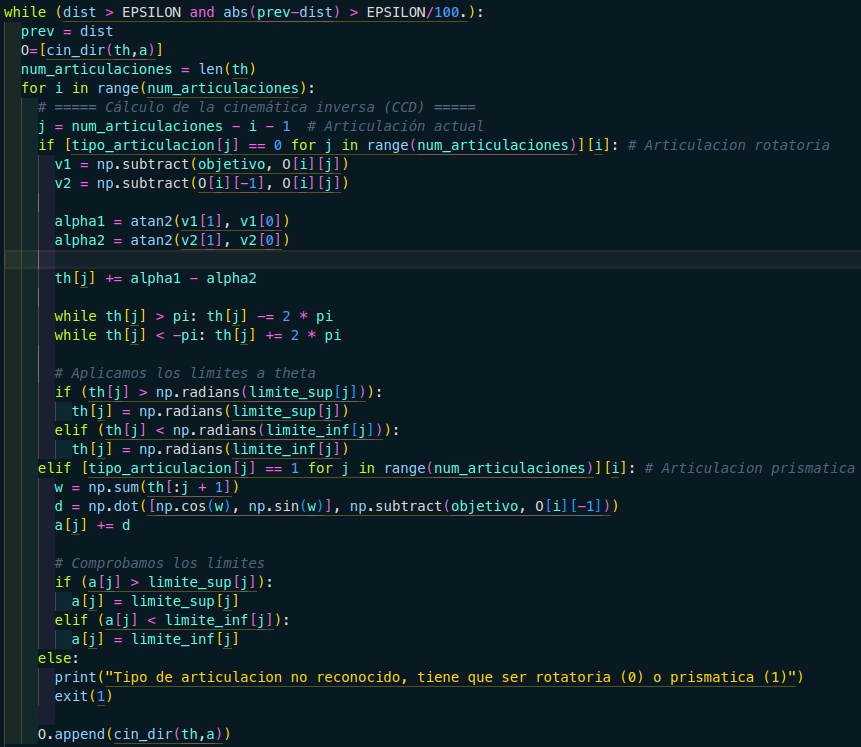
\includegraphics[scale=0.55]{img/codigo_ci_ccd.png}
  \caption{Inverse kinematics code with the CCD algorithm}
\end{figure}

\newpage

\section{Example execution}
An example of executing inverse kinematics script would be to move the robot to the point x = 5, y = 5:
\begin{figure}[H]
  \centering
  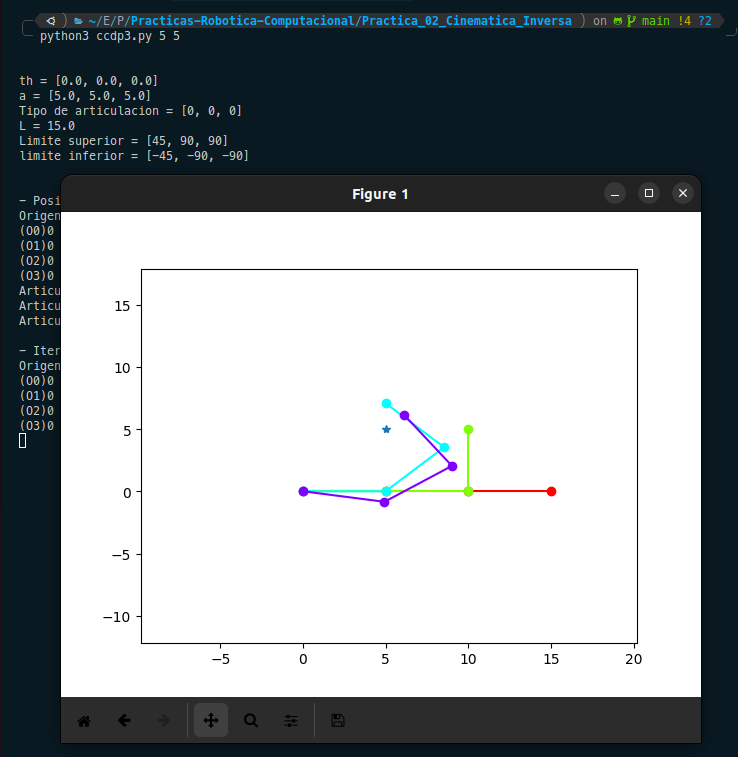
\includegraphics[scale=0.35]{img/ejemplo_ci_1.png}
  \caption{Example of the execution of inverse kinematics in the first iteration}
\end{figure}

\begin{figure}[H]
  \centering
  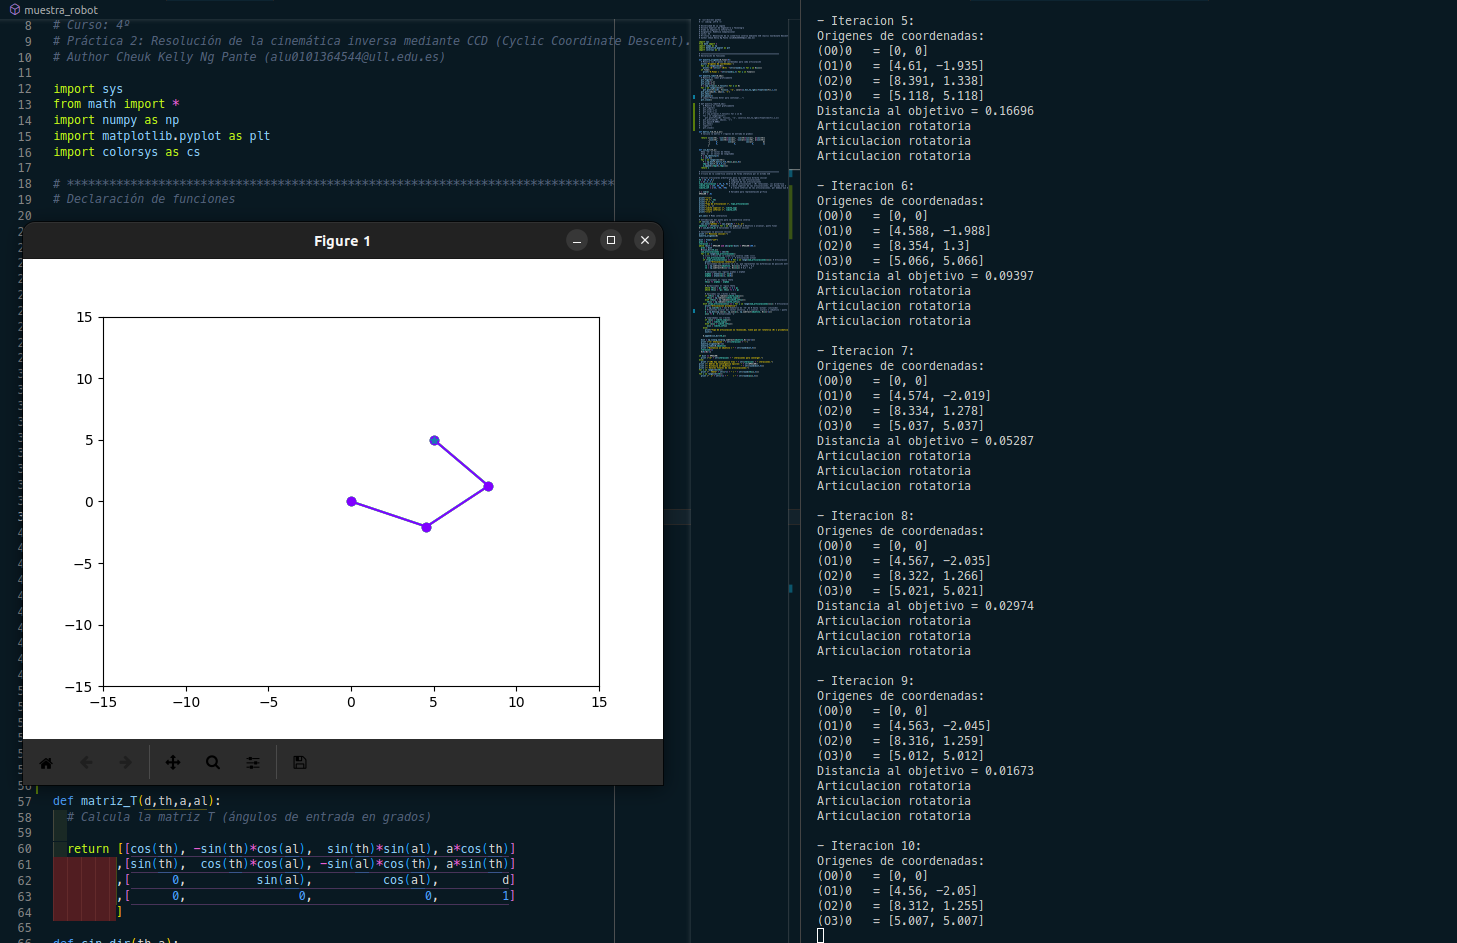
\includegraphics[scale=0.25]{img/ejemplo_ci_2.png}
  \caption{Example of inverse kinematics execution in the last iteration}
\end{figure}

\chapter{Localization}
Localization is the process of estimating the position of a robot in an unknown environment. Localization is a fundamental problem in mobile robotics, as most mobile robotics tasks require the robot to know its position in the environment. Localization is a difficult problem because the robot does not know its initial position and the environment may be unknown and dynamic. In addition, the robot's sensors may be noisy and the robot may have inaccurate movement.

In the practice of localization, the most probable position of the robot has to be calculated from its sensory system 
within a square region of centre "centre" and side $2 \cdot \text{radius}$.

To calculate the location in the script in \emph{Python} is to complete the function \emph{localizacion} which receives as parameters the beacons, the actual location of the robot, the ideal location of the robot, the centre of the region and the radius of the region and a show parameter to display the location graph. This function aims to find the most probable location of a robot within a square region, using its sensory system and a set of reference beacons.

The localization process is performed by comparing the measurements of the real robot with the measurements of the ideal robot at different points within the square region. The ideal robot is moved to each point and the error between the measurements of the ideal robot and the measurements of the real robot is calculated. The point with the smallest error is considered the most likely location of the real robot.

The code uses a \emph{for} loop to iterate over the points within the square region. It uses the function \emph{np.arange} to generate a sequence of values within the range of the radius of the region. This function returns an array of values that are used to calculate the `x` and `y` coordinates of the current point.

Within the loop, the position of the ideal robot is updated to the current point and the error between the measurements of the ideal robot and the measurements of the real robot is calculated using the function
\emph{real.measurement\_prob(ideal.sense(balizas), balizas)}. The error is stored in an image matrix.

The code also keeps track of the minimum error found so far and the point corresponding to that minimum error. If an error smaller than the current minimum error is found, the minimum error is updated and the current point is saved as the best point.

Once the loop is completed, the ideal robot is placed at the best point found, which is considered the most likely location of the actual robot. 
actual robot. Finally, the best point and the minimum error are printed.

Once the function \emph{localizacion} has been developed, it has been invoked before iterating over the list of target points and also at the end of the loop 
to relocate the robot to calculate the best position for the ideal robot based on the position of the real robot.

\newpage

\section{Localization code}

\begin{figure}[H]
  \centering
  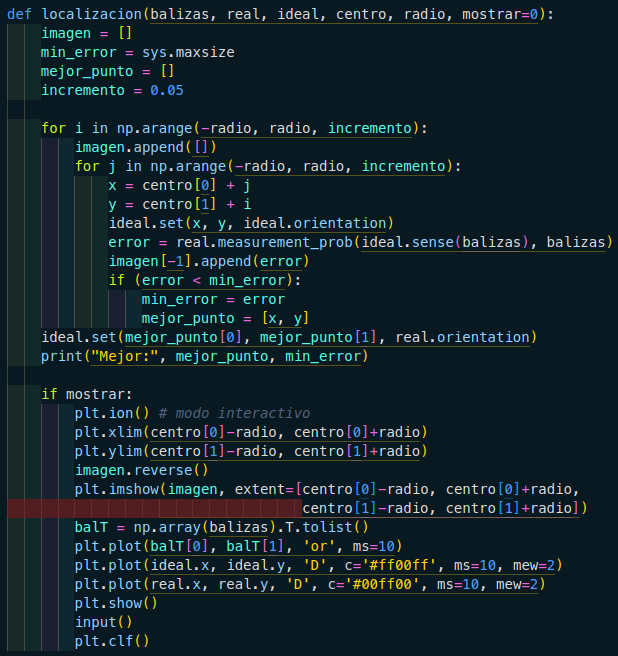
\includegraphics[scale=0.42]{img/localizacion.png}
  \caption{Localization code}
\end{figure}

\begin{figure}[H]
  \centering
  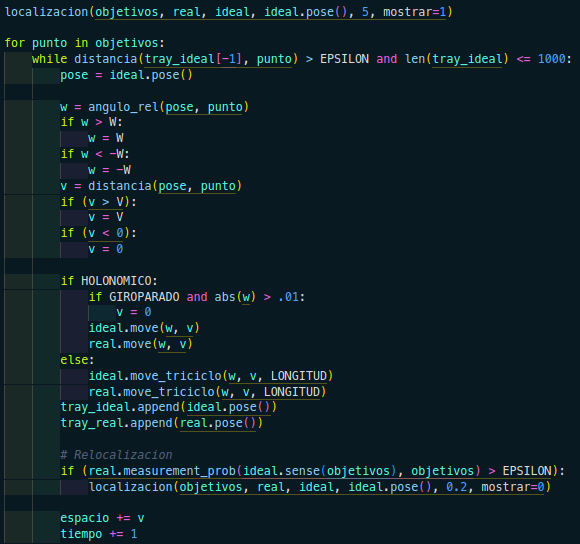
\includegraphics[scale=0.45]{img/localizacion_objetivos.png}
  \caption{Target localization code}
\end{figure}

\newpage

\section{Example execution}
\begin{figure}[H]
  \centering
  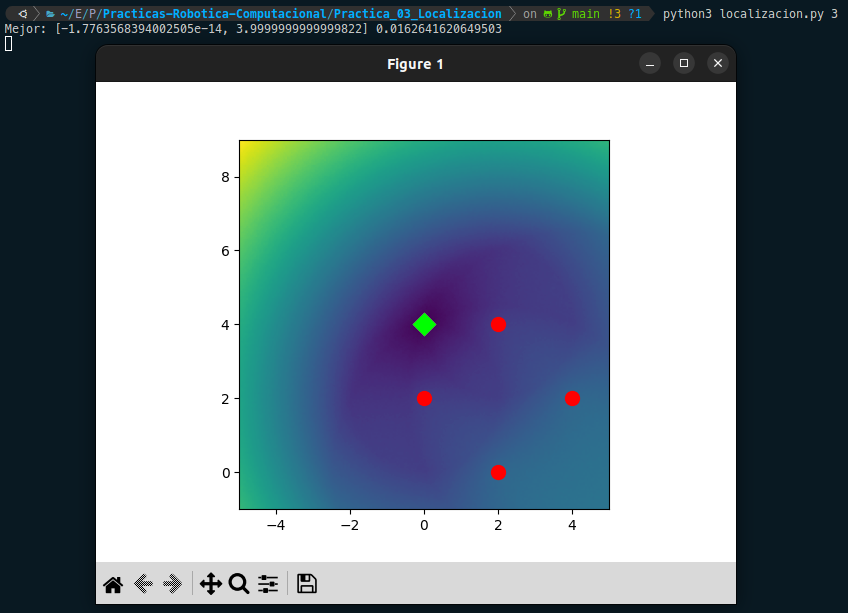
\includegraphics[scale=0.42]{img/localizacion_0.png}
  \caption{Example of localization execution}
\end{figure}

\begin{figure}[H]
  \centering
  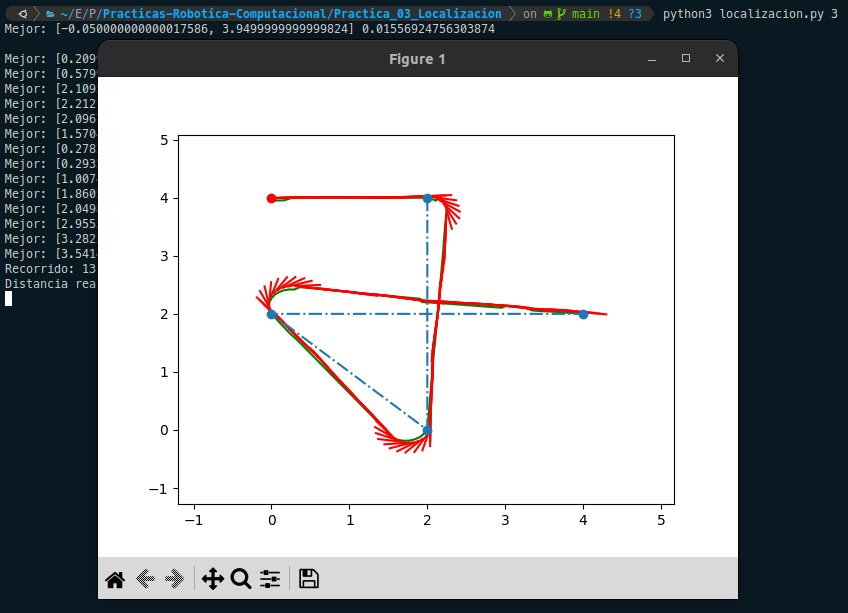
\includegraphics[scale=0.42]{img/localizacion_1.png}
  \caption{Example of localization execution}
\end{figure}

\end{document}